\documentclass{article}

\usepackage[utf8]{inputenc}
\usepackage{microtype}
\usepackage{geometry}

\usepackage{amsmath}
\usepackage{graphicx}
\usepackage{tikz}

\usepackage{enumitem}
\setlist{topsep=1ex}

\usepackage[font={sf}, labelfont={bf},
  labelsep=period, singlelinecheck=off]{caption}
\usepackage[font={sf}]{floatrow}
\usepackage{tabularx}

\usepackage[noblocks]{authblk}
\renewcommand{\Authsep}{, }
\renewcommand{\Authand}{ \& }
\renewcommand{\Authands}{ \& }
\renewcommand{\Affilfont}{\small}

\usepackage[pdfborder={0 0 0}]{hyperref}

\usepackage[style=science, article-title=true, maxnames=100]{biblatex}
\addbibresource{supplementary_text.bib}
\newcommand{\labeltitlepunc}{}
\DeclareBibliographyDriver{incollection}{%
  \usebibmacro{bibindex}%
  \usebibmacro{begentry}%
  \usebibmacro{author/translator+others}%
  \setunit{\labelnamepunct}\newblock
  \printlist{language}%
  \newunit\newblock
  \usebibmacro{byauthor}%
  \newunit\newblock
  \usebibmacro{title}%
  \usebibmacro{in:}%
  \usebibmacro{maintitle+booktitle}%
  \newunit\newblock
  \usebibmacro{byeditor+others}%
  \newunit\newblock
  \printfield{volumes}%
  \newunit\newblock
  \printfield{note}%
  \newunit\newblock
  \usebibmacro{publisher+location+date}%
  \newunit\newblock
  \printfield{volume}
  \newunit
  \usebibmacro{chapter+pages}%
  \newunit\newblock
  \iftoggle{bbx:isbn}
    {\printfield{isbn}}
    {}%
  \newunit\newblock
  \usebibmacro{doi+eprint+url}%
  \newunit\newblock
  \usebibmacro{addendum+pubstate}%
  \setunit{\bibpagerefpunct}\newblock
  \usebibmacro{pageref}%
  \newunit\newblock
  \usebibmacro{related}%
  \usebibmacro{finentry}%
}

\newcommand{\comment}[1]{\textbf{[#1]}}
\newcommand{\md}{\mathrm{d}}
\newcommand{\mT}{\mathrm{T}}
\renewcommand{\vec}[1]{\mathbf{#1}}
\newcommand{\mat}[1]{\mathbf{#1}}
\newcommand{\me}{\mathrm{e}}
\DeclareMathOperator{\Uniform}{Uniform}
\DeclareMathOperator{\Triangular}{Triangular}
\DeclareMathOperator{\Lognormal}{Lognormal}
\DeclareMathOperator{\BetaPERT}{Beta-PERT}

\newcommand{\labelPrefix}{S}
\renewcommand{\thesection}{\labelPrefix\arabic{section}}
\renewcommand{\theequation}{\labelPrefix\arabic{equation}}
\renewcommand{\thefigure}{\labelPrefix\arabic{figure}}
\renewcommand{\thetable}{\labelPrefix\arabic{table}}
\renewcommand{\figurename}{Fig.}


\title{Supporting online material for\\
  \emph{Effectiveness of UNAIDS targets and HIV vaccination across 127
    countries}}

\author[1*]{Jan Medlock}
\author[2]{Abhishek Pandey}
\author[2]{Alyssa S.~Parpia}
\author[2]{Amber Tang}
\author[2]{Laura A.~Skrip}
\author[2]{Alison P.~Galvani}
\affil[1]{Department of Biomedical Sciences, Oregon State University,
  106 Dryden Hall, Corvallis, OR, 97331-4801, USA}
\affil[2]{Center for Infectious Disease Modeling and Analysis, Yale
  School of Public Health, 135 College Street, New Haven, USA}
\affil[*]{To whom correspondence should be addressed.  E-mail:
  \href{mailto:jan.medlock@oregonstate.edu}{
    \texttt{jan.medlock@oregonstate.edu}}}


\begin{document}

\maketitle

The model simulation and analysis tools, written in Python, are
publicly available at\\
\url{https://github.com/janmedlock/HIV-95-vaccine/}
\cite{medlock2016-git}.


\section{Mathematical model}
\label{model}

We developed a country-level continuous-time, compartmental model that
divides people aged $15$\;y and older into non-overlapping HIV states.
We chose to consider only these ages because they are the vast
majority of global PLHIV, 93\% in 2014 \cite{UNICEF}; because
population-level HIV estimates and demographic data are often
stratified into ages $15$--$49$; and to capture the continuing burden
of infections in people ages $50$ and older.

The background mortality rate ($\mu$) in each of the
127 countries was collected from published estimates
\cite{World_Development_Indicators2013-ee}.  The recruitment rate
($\kappa$) into the age $15\;\text{y}$ and older group was set by the
difference between the country's population growth rate
\cite{WorldBankpg} and its background mortality rate
\cite{World_Development_Indicators2013-ee}, as would be true if the
population was at its stable age structure.

Our model has 8 HIV states (\autoref{model_diag}): susceptible to HIV
infection ($S$ is the number of people susceptible), vaccinated
against HIV ($R$), acute HIV infection ($A$), undiagnosed HIV
infection ($U$), diagnosed but untreated HIV infection ($D$), treated
without viral suppression ($T$), viral suppression ($V$), and having
AIDS ($W$).  Viral suppression is defined as a viral load of less than
1000 viral RNA copies per mL of blood.  Viral suppression not only
extends survival but also dramatically reduces transmission
\cite{vernazza2000, ioannidis2001, attia2009, May2014-gp}.
Transitions between model states are governed by a series of
differential equations parametrized using values found in other
studies, along with transmission rates derived from UNAIDS estimates
of incidence and prevalence (\autoref{model_param}).  The model is
deterministic, but uncertainty in the parameters is treated by running
the model 1000 times with samples from the parameter distributions
(\autoref{uncertainty}) and summarizing the model outcomes using the
median, 1st and 3rd quartiles (i.e., 25th and 75th percentiles), and
5th and 95th percentiles.  Each country was modeled separately
(\hyperref[effectiveness_Afghanistan]{Figures
  \ref*{effectiveness_Afghanistan}}--\ref{effectiveness_Zimbabwe}) and
the country simulations were aggregated to calculate global and
regional outcomes
(\hyperref[effectiveness_Global]{Figures
  \ref*{effectiveness_Global}}--\ref{effectiveness_Western_Europe}).

\begin{figure}
  \centering
  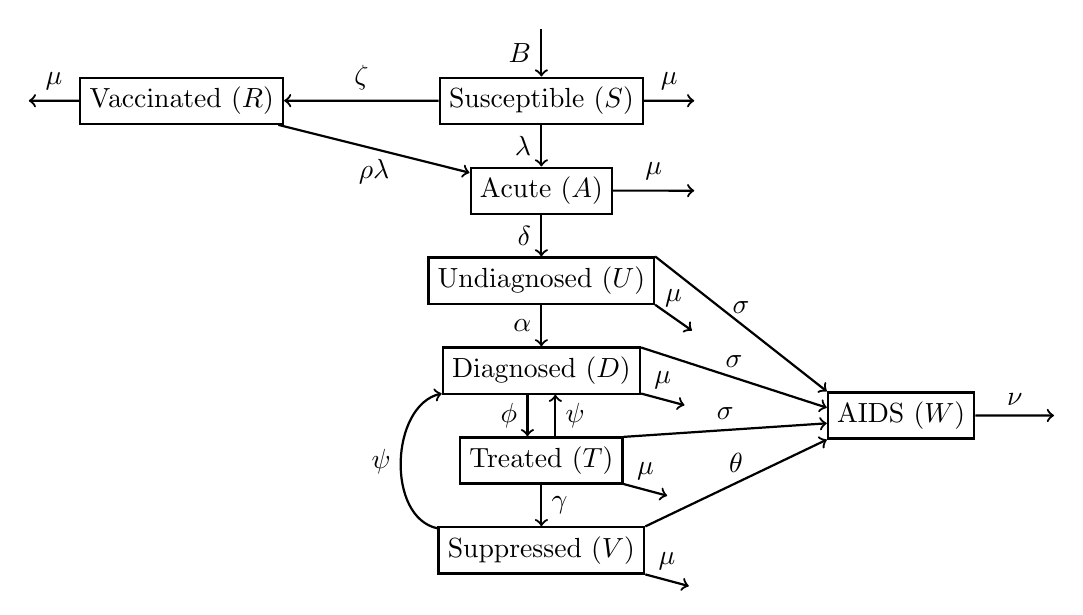
\begin{tikzpicture}[
  thick,
  scale = 1.142,
  compartment/.style = {draw},
  ]

  \node at (0, 5)
  [compartment, name = Susceptible] {Susceptible ($S$)};

  \node at (-4, 5)
  [compartment, name = Vaccinated] {Vaccinated ($R$)};

  \node at (0, 4)
  [compartment, name = Acute] {Acute ($A$)};

  \node at (0, 3)
  [compartment, name = Undiagnosed] {Undiagnosed ($U$)};

  \node at (0, 2)
  [compartment, name = Diagnosed] {Diagnosed ($D$)};

  \node at (0, 1)
  [compartment, name = Treated] {Treated ($T$)};

  \node at (0, 0)
  [compartment, name = Suppressed] {Suppressed ($V$)};

  \node at (4, 1.5)
  [compartment, name = AIDS] {AIDS ($W$)};

  \draw [->] (Susceptible) to node [left] {$\lambda$} (Acute);

  \draw [->] (Susceptible) to node [above] {$\zeta$} (Vaccinated);

  \draw [->] (Vaccinated) to node [below] {$\rho \lambda$} (Acute);

  \draw [->] (Acute) to node [left] {$\delta$} (Undiagnosed);

  \draw [->] (Undiagnosed) to node [left] {$\alpha$} (Diagnosed);

  \draw [->] (Diagnosed.240) to node [left] {$\phi$} (Treated.120);

  \draw [->] (Treated.60) to node [right] {$\psi$} (Diagnosed.300);

  \draw [->] (Treated) to node [right] {$\gamma$} (Suppressed);

  \draw [->] (Suppressed) to [out = 168, in = 193] node [left] {$\psi$} (Diagnosed);

  \draw [->] (Undiagnosed.12) to node [above] {$\sigma$} (AIDS.162);

  \draw [->] (Diagnosed.13) to node [above] {$\sigma$} (AIDS.174);

  \draw [->] (Treated.16) to node [above] {$\sigma$} (AIDS.186);

  \draw [->] (Suppressed.13) to node [above] {$\theta$} (AIDS.198);

  \draw [<-] (Susceptible) to node [left] {$B$} +(90: 0.8);

  \draw [->] (Susceptible) to node [above] {$\mu$} +(0: 1.7);

  \draw [->] (Vaccinated) to node [above] {$\mu$} +(0: -1.7);

  \draw [->] (Acute) to node [above] {$\mu$} +(0: 1.7);

  \draw [->] (Undiagnosed.348) to node [above] {$\mu$} +(325: 0.5);

  \draw [->] (Diagnosed.347) to node [above] {$\mu$} +(345: 0.5);

  \draw [->] (Treated.344) to node [above] {$\mu$} +(345: 0.5);

  \draw [->] (Suppressed.347) to node [above] {$\mu$} +(345: 0.5);

  \draw [->] (AIDS) to node [above] {$\nu$} +(0: 1.7);

\end{tikzpicture}


%%% Local Variables:
%%% mode: latex
%%% TeX-master: "model"
%%% End:

  \caption{Model diagram.}
  \label{model_diag}
\end{figure}

\begin{table}
  \begin{center}
    \begin{tabularx}{\textwidth}{lXlll}
      \hline
      & Definition & Value & Reference \\
      \hline
      $\mu$ & Background death rate & Country specific, Table S2
      & \cite{World_Development_Indicators2013-ee} \\
      $\kappa$ & Recruitment rate & Country specific, Table S2
      & \cite{World_Development_Indicators2013-ee, WorldBankpg} \\
      $\delta$	& Rate of leaving acute infection
      & $\Triangular$(2, 4.14, 9.6)\;y$^{-1}$
      & \cite{Hollingsworth2008-iy} \\
      $\sigma$	& Rate of developing AIDS without viral suppression
      & 0.1064\;y$^{-1}$ & \cite{Morgan2002-cq} \\
      $\theta$ & Rate of developing AIDS with viral suppression
      & Eq.~(\ref{theta}) & --- \\
      $\gamma$ & Rate of viral suppression
      & $\Uniform$(0.5, 1.5)\;y$^{-1}$
      & \cite{Currie2009-yz} \\
      $\nu$ & Death rate from AIDS & 0.5\;y$^{-1}$
      & \cite{Morgan2002-cq} \\
      $\rho$ & Vaccine efficacy & 50\%\,[30\%, 70\%] & --- \\
      $\omega$	& Reduction in lifetime with viral suppression
      & $\Uniform$(5, 8)\;y
      & \cite{Samji2013-kf, Unaids2014-ue} \\
      $\tau_{A}$ & Transmissibility during acute phase
      & $\Triangular$(0.0039, 0.0082, 0.0150)
      & \cite{Wawer2005-us, Skarbinski2015-ni}\\
      $\tau_{U}$ & Transmissibility after acute phase
      & $\Triangular$(0.00077, 0.0014, 0.00251)
      & \cite{Hughes2012-so} \\
      $\varepsilon$ & Relative transmissibility with
      viral suppression & $\BetaPERT$(0.08, 0.002, 0.57)
      & \cite{Donnell2010-xo} \\
      $n$ & Coital acts per year & $\Uniform$(96, 108)
      & \cite{Wawer2005-us, Abdool_Karim2010-cm}\\
      $\alpha$ & Diagnosis rate & See eq.~(\ref{diagnosis_rate}) & --- \\
      $\phi$ & Treatment rate & See eq.~(\ref{treatment_rate}) & --- \\
      $\psi$ & Rate of relapse to untreated & See eq.~(\ref{relapse_rate})
      & --- \\
      $\zeta$ & Vaccination rate & See eq.~(\ref{vaccination_rate}) & --- \\
      \hline
    \end{tabularx}
    \caption{Model parameters. $\Triangular$, $\Uniform$, and
      $\BetaPERT$ are sampling distributions: see
      \autoref{uncertainty} for a full description.  For vaccine
      efficacy, $50\%$ was the baseline, and $30\%$ and $70\%$ were
      also used in a scenario analysis.}
    \label{model_param}
  \end{center}
\end{table}

People susceptible to HIV ($S$) progress to acute infection ($A$)
according to the force of infection ($\lambda$,
eq.~\eqref{force_of_infection}), which depends on the HIV transmission
rate, estimated from the country-specific incidence and prevalence
data (\autoref{model_fitting}), adjusted for the current number of
acutely infected, untreated or ineffectively treated, and viral
suppression PLHIV.  Acute infection is characterized by high viral
loads and lasts an average of 2.90 [95\% confidence interval 1.23,
6.00]\;months \cite{Hollingsworth2008-iy}.  (We converted these
durations to rates like $1 / 2.90\;\text{month$^{-1}$} \approx
4.14\;\text{y$^{-1}$}$ and set the parameter using random samples from
$\Triangular(2, 4.14, 9.6)\;\text{y$^{-1}$}$ to capture the
uncertainty in its value.  See \autoref{uncertainty} for the
definition of $\Triangular(a, b, c)$ and other distributions.)  We
assumed that people remain undiagnosed during their acute-infection
phase. After acute infection, people move into the chronic undiagnosed
class ($U$).  People in the undiagnosed class will be diagnosed at the
rate $\alpha$, which is determined by the country's current diagnosis
level and its diagnosis target (\autoref{targets}).  Diagnosed people
($D$) transition to the treated compartment ($T$) upon starting ART at
the rate $\phi$, dependent on the country's current treatment level
and its treatment target (\autoref{targets}).  After some time,
treated people then transition to the viral-suppression class ($V$),
at the rate $\gamma$.  We took $\gamma$ as a random sample from
$\Uniform(0.5, 1.5)\;\text{y$^{-1}$}$, that is, viral suppression
occurs after between 8 months and 2 years on treatment
\cite{Currie2009-yz}.  Disengagement from treatment moves people from
treated ($T$) and viral suppression ($V$) at the rate $\psi$,
dependent on the current level of viral suppression and the country's
target (\autoref{targets}), back to the diagnosed class ($D$).

PLHIV without viral suppression (compartments $U$, $D$, and $T$)
develop AIDS (compartment $W$) after an average duration of 10.4 y
\cite{Morgan2002-cq}, i.e., with transition rate
$\sigma = 0.1064\;\text{y$^{-1}$}$.  People who have achieved viral
suppression ($V$) develop AIDS at rate $\theta$, slower than PLHIV
without viral suppression.  People with viral suppression are
estimated to live $5$--$8$\;y shorter lives than the non-HIV infected
\cite{Samji2013-kf, Unaids2014-ue}, which we quantified by randomly
sampling the parameter $\omega$ from $\Uniform(5, 8)\;\text{y}$.
Assuming no relapse to untreated, the duration of viral suppression is
\begin{equation}
  \frac{1}{\theta + \mu} = \frac{1}{\mu} - \omega - \frac{1}{\nu}.
\end{equation}
The term to the left of the equals sign is the time until leaving
viral suppression by either progression to AIDS (at rate $\theta$) or
background mortality (at rate $\mu$).  The term to the right of the
equals sign is the lifespan of the non-HIV infected, minus the
reduction in life due to having HIV with viral suppression, minus the
duration of the AIDS stage.  Solving for $\theta$ gives the rate of
progression to AIDS with viral suppression as
\begin{equation}
  \label{theta}
  \theta = \frac{1}{1/\mu - \omega - 1/\nu} - \mu.
\end{equation}

In scenarios with vaccine, susceptible people are vaccinated at rate
$\zeta$, depending on the country's current vaccination coverage and
its coverage target (\autoref{targets}), transitioning into the
vaccinated compartment ($R$), where the vaccine reduces their force of
infection by the efficacy factor $\rho$.  We took the base-case
efficacy to be $50\%$ and varied it to $30\%$ and $70\%$ in analyzing
vaccination scenarios (\autoref{uncertainty}).  We did not model
specific vaccine dose regime, such that implicit in our efficacy
parameter is the assumption that boosters will be used to maintain
efficacy over time.  Without vaccine, $\zeta = 0$.

We also added differential equations to track the cumulative number of
new infections ($Y$) and AIDS deaths ($Z$) over the model period.

The model equations are
\begin{equation}
  \label{model_eqns}
  \begin{split}
    \frac{\md S}{\md t} &= \kappa N - \lambda S - \zeta S- \mu S,
    \\
    \frac{\md R}{\md t} & = \zeta S - (1 - \rho) \lambda R - \mu R,
    \\
    \frac{\md A}{\md t} &= \lambda S + (1 - \rho) \lambda R - \delta A - \mu A,
    \\
    \frac{\md U}{\md t} &= \delta A - \alpha U - \mu U - \sigma U,
    \\
    \frac{\md D}{\md t} &=  \alpha U + \psi T + \psi V
    - \phi D - \mu D - \sigma D,
    \\
    \frac{\md T}{\md t} &= \phi D - \psi T - \gamma T - \mu T
    - \sigma T,
    \\
    \frac{\md V}{\md t} &= \gamma T - \psi V - \mu V - \theta V,
    \\
    \frac{\md W}{\md t} &= \sigma U + \sigma D + \sigma T + \theta V -
    \nu W,
    \\
    \frac{\md Y}{\md t} &= \lambda \big[S + (1 - \rho) R\big],
    \\
    \frac{\md Z}{\md t} &= \nu W,
  \end{split}
\end{equation}
with force of infection
\begin{equation}
  \label{force_of_infection}
  \lambda =
  \frac{\eta \big[\beta_A A + \beta_U (U + D + T) + \beta_V V\big]}{N},
\end{equation}
sexually active population size $N = S + R + A + U + D + T + V$.  We
assumed that people with AIDS ($W$) are too sick to be sexually
active.

The relative transmission rates of acute, unsuppressed, and suppressed
infected people are
\begin{equation}
  \label{betas}
  \begin{split}
    \beta_A &= 1 - (1 - \tau_A)^n,
    \\
    \beta_U &= 1 - (1 - \tau_U)^n,
    \\
    \beta_V &= 1 - (1 - \varepsilon \tau_U)^n,
  \end{split}
\end{equation}
where the $\tau$'s are the relative transmissibilities of people with
acute ($A$), unsuppressed ($U$ and $T$), and suppressed ($V$)
infections, $n$ is the annual number of coital acts, and $\varepsilon$
is the relative transmissibility with viral suppression.  For
transmissibility during the acute phase, we sampled $\tau_A$ from
$\Triangular$(0.0039, 0.0082, 0.0150)
\cite{Wawer2005-us, Skarbinski2015-ni}, whereas, for transmissibility
for unsuppressed people, we sampled $\tau_U$ from
$\Triangular(0.00077, 0.0014, 0.00251)$ \cite{Hughes2012-so}.  The
transmissibility of people with viral suppression relative to those
without suppression has been estimated at 0.08 (95\% confidence
interval 0.002, 0.57) \cite{Donnell2010-xo}: due to the extremely long
left tail, we chose to sample the relative transmissibility
$\varepsilon$ from $\BetaPERT(0.08, 0.002, 0.57)$ rather than a
$\Triangular$ distribution.  (See \autoref{uncertainty} for a full
description of $\BetaPERT(a, b, c)$.)  The annual number of coital
acts $n$ was sampled from $\Uniform(96, 108)$
\cite{Wawer2005-us, Abdool_Karim2010-cm}.  The country-specific
transmission rate $\eta$ was derived from UNAIDS estimates of each
country's longitudinal HIV prevalence and incidence
(\autoref{model_fitting}).

For year 2015, estimates of the number of people aged 15--49 years,
$M(2015)$; the prevalence, $p_I(2015)$; the proportion diagnosed,
$p_D(2015)$; the proportion treated, $p_T(2015)$; and proportion with
viral suppression, $p_V(2015)$ were used to initialize the model
(\autoref{data_sources}).  Although the initial population used ages
15--49 due to the availability of published estimates, model
projections allowed for analysis of infected people aging beyond age
50.  Due to a lack of published estimates of acute infections, and
since the acute phase is so much shorter than the other stages, we
assumed that initially there were no acute infections.  Due to a lack
of comprehensive estimates of the number of people with AIDS in each
country, we assumed that the proportion of diagnosed, untreated people
($D + W$) who have AIDS ($W$) in year 2015 was
\begin{equation}
  p_A = \frac{\sigma}{\sigma + \nu},
\end{equation}
which is the equilibrium fraction of diagnosed people ($D + W$) who
have AIDS ($W$) in the absence of treatment and background mortality.
The number initially vaccinated was set to 0.  The initial cumulative
number of new infections and AIDS deaths were set to 0.  Thus, the
model initial conditions are
\begin{equation}
  \label{initial_conditions}
  \begin{split}
    S(2015) &= \big(1 - p_I(2015)\big) M(2015), \\
    R(2015) &= 0, \\
    A(2015) &= 0, \\
    U(2015) &= \big(1 - p_D(2015)\big) p_I(2015) M(2015), \\
    D(2015) &= \big(1 - p_A\big) p_D(2015) \big(1 - p_T(2015)\big)
    p_I(2015) M(2015), \\
    T(2015) &= p_D(2015) p_T(2015) \big(1 - p_V(2015)\big)
    p_I(2015) M(2015), \\
    V(2015) &= p_D(2015) p_T(2015) p_V(2015) p_I(2015) M(2015), \\
    W(2015) &= p_A p_D(2015) \big(1 - p_T(2015)\big) p_I(2015) M(2015), \\
    Y(2015) &= 0, \\
    Z(2015) &= 0.
  \end{split}
\end{equation}

The parametrized differential equations were solved numerically
\cite[see][]{medlock2016-git} and four effectiveness outcomes were
computed from the solutions.
\begin{description}
\item[New infections] New infections from 2015 to time $t$ are given
  by $Y(t)$.

\item[Per-capita incidence] At each solution time point, the
  per-capita incidence was calculated as
  \begin{equation}
    i(t_j) = \frac{Y(t_j) - Y(t_{j - 1})}{M(t_j) (t_j - t_{j - 1})},
  \end{equation}
  where
  \begin{equation}
    M(t) = S(t) + R(t) + A(t) + U(t) + D(t) + T(t) + V(t) + W(t)
  \end{equation}
  is the total population size at time $t$.  The per-capita incidence
  at the first time point was undefined.

\item[PLHIV] At each solution time point, PLHIV was given by
  \begin{equation}
    A(t) + U(t) + D(t) + T(t) + V(t) + W(t).
  \end{equation}

\item[AIDS-related deaths] AIDS-related deaths from 2015 to time $t$
  are given by $Z(t)$.

\end{description}

The results from the country simulations were aggregated to the
regional and global levels by adding the numbers of people in each
compartment over time and then new infections, per-capita incidence,
PLHIV, and HIV-related deaths were calculated from the aggregates.
(See Table S6 for the definitions of UNAIDS regions.)


\section{Target rates}
\label{targets}

The current proportion of PLHIV who know their diagnosis is
\begin{equation}
  p_D(t) = \frac{D(t) + T(t) + V(t) + W(t)}
  {A(t) + U(t) + D(t) + T(t) + V(t) + W(t)},
\end{equation}
and the desired target for the current level of diagnosis is
$p_D^*(t)$.  For the rate of new diagnosis, we used the function
\begin{equation}
  \label{diagnosis_rate}
  \alpha(t) = \alpha_{\max} H\big(p_D^*(t) - p_D(t)\big),
\end{equation}
where $H(x)$ is the Heaviside-like function
\begin{equation}
  H(x) =
  \begin{cases}
    0 & \text{if $x < 0$},
    \\
    x / \chi & \text{if $0 \leq x \leq \chi$},
    \\
    1 & \text{if $x > \chi$},
  \end{cases}
\end{equation}
with $\chi = 0.001$, which rapidly switches from $H = 0$ when $x < 0$
to $H = 1$ when $x > 0$.  The linear segment connecting $H = 0$ and
$H = 1$ was used to avoid difficulties in computing numerical
solutions that occur when using a discontinuous function.  The
function for the rate of new diagnoses \eqref{diagnosis_rate} allows
new diagnoses ($\alpha(t) > 0$) when the current diagnosis level is
below the target ($p_D^*(t) > p_D(t)$), and stops new
diagnoses ($\alpha(t) = 0$) when the current diagnosis level is at or
above target.  We took $\alpha_{\max} = 1\;\text{y$^{-1}$}$.

The proportion of diagnosed people who are treated is
\begin{equation}
  p_T(t) = \frac{T(t) + V(t) + W(t)}{D(t) + T(t) + V(t) + W(t)}.
\end{equation}
Like the rate of new diagnosis, the rate of enrolling new people in
treatment is
\begin{equation}
  \label{treatment_rate}
  \phi(t) = \phi_{\max} H\big(p_T^*(t) - p_T(t)\big),
\end{equation}
with $\phi_{\max} = 10$, allowing new treatment ($\phi(t) > 0$) when
the current treatment level is below the target ($p_T^*(t) > p_T(t)$)
and stopping new treatment ($\phi(t) = 0$) when the current treatment
level is at or above target.

The proportion of people on ART who have achieved viral suppression is
\begin{equation}
  p_V(t) = \frac{V(t)}{T(t) + V(t)}.
\end{equation}
The rate of people relapsing to untreated is
\begin{equation}
  \label{relapse_rate}
  \psi(t) = \psi_{\max} H\big(p_V(t) - p_V^*(t)\big),
\end{equation}
with $\psi_{\max} = 1$, which, unlike diagnosis and treatment rates,
prevents relapses ($\psi(t) = 0$) when the current level of viral
suppression is below the target ($p_V^*(t) > p_V(t)$) and allows
relapses ($\psi(t) > 0$) when the current level of viral suppression
is at or above target.  We chose to vary the relapse rate to achieve
the desired level of viral suppression because achieving viral
suppression seems to depend on the time on treatment (i.e.,
$1 / \gamma$), while relapse rates are difficult to estimate.

The proportion of susceptible people vaccinated is
\begin{equation}
  p_R(t) = \frac{R(t)}{S(t) + R(t)}.
\end{equation}
Like diagnosis and treatment, the vaccination rate is
\begin{equation}
  \label{vaccination_rate}
  \zeta(t) = \zeta_{\max} H\big(p_R^*(t) - p_R(t)\big),
\end{equation}
with $\zeta_{\max} = 1$, allowing vaccination ($\zeta(t) > 0$) when
the current vaccine coverage level is below the target
($p_R^*(t) > p_R(t)$) and stopping vaccination ($\zeta(t) = 0$) when
the current vaccine coverage is at or above target.

We modeled 3 different targets for the proportion diagnosed ($p_D$), the
proportion treated ($p_T$), and the proportion with viral suppression ($p_V$).
\begin{description}
\item[Status quo] The status quo target is for the proportions $p_D$,
  $p_T$, and $p_V$ to remain fixed at their initial levels (Table S5)
  going forward. That is,
  \begin{equation}
    \label{status_quo_target}
    \begin{split}
      p_D^*(t) &= p_D(2015), \\
      p_T^*(t) &= p_T(2015), \\
      p_V^*(t) &= p_V(2015).
    \end{split}
  \end{equation}

\item[UNAIDS 90--90--90] The UNAIDS 90--90--90 target is for $p_D$,
  $p_T$, and $p_V$ to all be raised to $90\%$ by 2020.  We implemented
  this target as linear increases from the 2015 levels, each up to
  $90\%$ in 2020, and constant at $90\%$ from 2020 to 2035, except if
  an initial level is above $90\%$ then it remains constant from 2015
  to 2035 so that meeting the UNAIDS target does not worsen any aspect
  of the treatment cascade.  That is,
  \begin{equation}
    \label{unaids90_targets}
    \begin{split}
      p_D^*(t) &=
      \begin{cases}
        F\big(t, 2015, p_D(2015), 2020, 0.9\big)
        & \text{if $p_D(2015) < 0.9$},
        \\
        p_D(2015) & \text{if $p_D(2015) \geq 0.9$}.
      \end{cases}
      \\
      p_T^*(t) &=
      \begin{cases}
        F\big(t, 2015, p_T(2015), 2020, 0.9\big)
        & \text{if $p_T(2015) < 0.9$},
        \\
        p_T(2015) & \text{if $p_T(2015) \geq 0.9$}.
      \end{cases}
      \\
      p_V^*(t) &=
      \begin{cases}
        F\big(t, 2015, p_V(2015), 2020, 0.9\big)
        & \text{if $p_V(2015) < 0.9$},
        \\
        p_V(2015) & \text{if $p_V(2015) \geq 0.9$}.
      \end{cases}
    \end{split}
  \end{equation}
  where
  \begin{equation}
    \label{F}
    F(t, t_0, x_0, t_1, x_1) =
    \begin{cases}
      x_0 & \text{if $t < t_0$},
      \\
      x_0 + (x_1 - x_0) \frac{t - t_0}{t_1 - t_0} &
      \text{if $t_0 \leq t < t_1$},
      \\
      x_1 & \text{if $t \geq t_1$},
    \end{cases}
  \end{equation}
  is constant at $x_0$ for $t < t_0$, linearly connects $x_0$ at
  $t_0$ to $x_1$ at $t_1$ for $t_0 \leq t < t_1$, and is constant at
  $x_1$ for $t \geq t_1$.

\item[UNAIDS 95--95--95] The UNAIDS 95--95--95 target is to achieve
  90--90--90 by 2020 and then for $p_D$, $p_T$, and $p_V$ to all be
  raised to $95\%$ by 2030.  We implemented this target as for
  90--90--90 from 2015 to 2020, and then linear increases from the
  2020 levels up to $95\%$ in 2030, again with the exception that if
  an initial level is above $95\%$ then it remains constant from 2015
  to 2035.  That is,
  \begin{equation}
    \label{unaids95_targets}
    \begin{split}
      p_D^*(t) &=
      \begin{cases}
        G\big(t, 2015, p_D(2015), 2020, 0.9, 2030, 0.95\big)
        & \text{if $p_D(2015) < 0.9$},
        \\
        F\big(t, 2020, p_D(2015), 2030, 0.95\big)
        & \text{if $0.9 \leq p_D(2015) < 0.95$},
        \\
        p_D(2015) & \text{if $p_D(2015) \geq 0.95$},
      \end{cases}
      \\
      p_T^*(t) &=
      \begin{cases}
        G\big(t, 2015, p_T(2015), 2020, 0.9, 2030, 0.95\big)
        & \text{if $p_T(2015) < 0.9$},
        \\
        F\big(t, 2020, p_T(2015), 2030, 0.95\big)
        & \text{if $0.9 \leq p_T(2015) < 0.95$},
        \\
        p_T(2015) & \text{if $p_T(2015) \geq 0.95$},
      \end{cases}
      \\
      p_V^*(t) &=
      \begin{cases}
        G\big(t, 2015, p_V(2015), 2020, 0.9, 2030, 0.95\big)
        & \text{if $p_V(2015) < 0.9$},
        \\
        F\big(t, 2020, p_V(2015), 2030, 0.95\big)
        & \text{if $0.9 \leq p_V(2015) < 0.95$},
        \\
        p_V(2015) & \text{if $p_V(2015) \geq 0.95$},
      \end{cases}
    \end{split}
  \end{equation}
  where
  \begin{equation}
    G(t, t_0, x_0, t_1, x_1, t_2, x_2) =
    \begin{cases}
      x_0 & \text{if $t < t_0$},
      \\
      x_0 + (x_1 - x_0) \frac{t - t_0}{t_1 - t_0} &
      \text{if $t_0 \leq t < t_1$},
      \\
      x_1 + (x_2 - x_1) \frac{t - t_1}{t_2 - t_1} &
      \text{if $t_1 \leq t < t_2$},
      \\
      x_2 & \text{if $t \geq t_2$},
    \end{cases}
  \end{equation}
  is constant at $x_0$ for $t < t_0$, linearly connects $x_0$ at $t_0$
  to $x_1$ at $t_1$ for $t_0 \leq t < t_1$, linearly connects $x_1$ at
  $t_1$ to $x_2$ at $t_2$ for $t_1 \leq t < t_2$, and is constant at
  $x_2$ for $t \geq t_2$, and $F$ is as in eq.~\eqref{F}.

\end{description}

For vaccination, we assume that rollout begins in year $t_V = 2020$
(or $t_V = 2025$ in vaccine scenario analysis, \autoref{uncertainty}),
that rollout linearly increases the proportion of the non-infected
population covered from 0\% by $r_V = 25\%$ per year (or $r_V = 10\%$
per year) up to $c_V = 70\%$ (or $c_V = 50\%$ or $c_V = 90\%$) and
staying constant thereafter.  Thus, the vaccination target is
\begin{equation}
  \label{vaccination_target}
  p_R^*(t) =
  \begin{cases}
    0 & \text{if $t < t_V$},
    \\
    r_V (t - t_V) & \text{if $t_V \leq t < T_V$},
    \\
    c_V & \text{if $t \geq T_V$},
  \end{cases}
\end{equation}
where $T_V = t_V + c_V / r_V$ is the time when rollout reaches
the ultimate coverage $c_V$.

Target strategies were one of the three diagnosis and treatment
targets (status quo, 90--90--90, or 95--95--95), combined with either
no vaccination ($p_R^*(t) = 0$) or vaccination at some level of
efficacy, ultimate coverage, start date of rollout, and speed of
rollout.


\section{Data sources}
\label{data_sources}

For 127 countries, we found sufficient published estimates and data to
parametrize our model.  Demographic data, including population growth
rate \cite{WorldBankpg}, death rate
\cite{World_Development_Indicators2013-ee}, and number of people aged
15--49 years \cite{The_World_Bank2016-fd} were obtained from the World
Bank (Table S2). Longitudinal HIV prevalence (Table S3) and incidence
(Table S4) estimates for ages 15--49, spanning from as early as 1990
to 2015, were primarily obtained from the AIDSinfo database produced
by UNAIDS \cite{Unaids2016-an}. Other sources included UNAIDS Country
Progress Reports \cite{Unaids2016-am} published from 2012 to 2016 and
AIDS Data Hub \cite{AIDSdatahub-fg}, which compiles data from UNAIDS,
UNICEF, WHO, and the Asian Development Bank. These sources were also
used to inform the initial conditions for the model: the number of
people diagnosed with HIV, the number on ART, and the number who have
viral suppression or have been retained on treatment for at least 12
months (Table S5). Where estimates or data were not available from
these sources, alternative resources such as peer-reviewed journal
articles and country health ministry reports were consulted.  See
Tables S2--S5 for full information on the sources used for each
country.  These source tables are also available in the public
source-code repository \cite{medlock2016-git}.


\section{Model fitting}
\label{model_fitting}

Using available historical country-level estimates of prevalence and
incidence (Tables S3 and S4), and published estimates of
transmissibility
\cite{Wawer2005-us,Donnell2010-xo,Hughes2012-so,Skarbinski2015-ni}, we
derived an average country-specific transmission rate, which then
informs the acute, unsuppressed, and suppressed transmission rates.
This calibration method provided a recent estimate of country-specific
transmission, while using historical data to smooth out short-term
variations.

For each country, we first derived time-dependent rates of HIV
transmission for each of the available points in the historical
estimates of prevalence and incidence.  The calculation involved
approximating the simplified force of infection
\begin{align}
  \label{foi}
  \begin{split}
    \lambda(t) &= \frac{\eta \left[\beta_{A} A(t)
        + \beta_{U} \big(U(t) + D(t) + T(t)\big) +
        \beta_{V} V(t)\right]}{N(t)}
    \approx  \beta(t) \frac{I(t)}{N(t)},
  \end{split}
\end{align}
where $\beta$ is the estimated time-dependent aggregate transmission
rate under the approximation that there is no difference in
transmission risk among acute, unsuppressed, suppressed, and AIDS
classes, and $I = A + U + D + T + V + W$ is the total number of PLHIV.
Therefore, the per-capita incidence is
\begin{equation}
i(t) = \lambda(t) \frac{S(t)}{N(t)}
\approx \beta(t) \frac{I(t)}{N(t)} \frac{S(t)}{N(t)} =\beta(t) p(t) (1-p(t)),
\end{equation}
where $p(t)$ is the prevalence. Thus, we calculated the transmission
rate at each historical time point using the incidence and prevalence
estimates by
\begin{equation}
  \label{trans_rate}
  \beta(t) \approx \frac{i(t)}{p(t)(1-p(t))}.
\end{equation}

To reflect the uncertainty in $\beta(t)$, we assumed that it follows a
lognormal distribution (\autoref{uncertainty}). For the parameters
$\mu$ and $\sigma^2$ of the lognormal distribution we used the
exponentially weighted mean and variance \cite{holt2004} over time
(with half-life 1\;y) of $\log \beta(t)$ for the year 2015.  That is,
\begin{equation}
  \label{lognormal_params}
  \begin{split}
    \mu &= \frac{\sum_{i = 1}^n  2^{t_i}
      \log \beta(t_i)}
    {\sum_{i = 1}^n 2^{t_i}},
    \\
    \sigma^2 &= \frac{\big(\sum_{i = 1}^n 2^{t_i}\big)
      \left[\sum_{i = 1}^n  2^{t_i}
        \big(\log \beta(t_i) - \mu\big)^2\right]}
    {\big(\sum_{i = 1}^n 2^{t_i}\big)^2
      - \sum_{i = 1}^n 2^{2 t_i}}.
  \end{split}
\end{equation}
A half-life of 1\;y means that the estimate of the transmission rate
from year $i$ is weighted half as much as the estimate from year
$i + 1$, a quarter as much as the estimate from year $i + 2$, and so
on.  This approach captured the recent country-level transmission
behavior while still allowing for the use of less-recent estimates to
smooth short-term variations (\autoref{transmission_rate}).

\begin{figure}
  \centering
  \includegraphics{../Codes/plots/transmission_rate.pdf}
  \caption{Country-specific distributions of transmission rate,
    $\bar{\beta}$, calculated based on UNAIDS historical estimates of
    country prevalence and incidence.  See \autoref{model_fitting}.}
  \label{transmission_rate}
\end{figure}

For each of the 1000 model parameter samples, the country-level
aggregate transmission rate $\bar{\beta}$ was sampled from
$\Lognormal(\mu, \sigma^2)$ with the parameters given by
eqs.~\eqref{lognormal_params}, and samples were also drawn for the
transmissibilities for acute and unsuppressed infected people,
$\tau_A$ and $\tau_U$; the transmission reduction by suppression,
$\varepsilon$; and the annual number of coital acts, $n$
(\autoref{model}).  From the latter samples, the relative transmission
rates for the acute phase ($\beta_A$), for unsuppressed chronic
infections ($\beta_U$), and for chronic infections with viral
suppression ($\beta_V$) were calculated by eqs.~\eqref{betas}.  The
sample value of the country-level transmission rate was then computed
by
\begin{equation}
  \label{eta}
  \eta = \frac{\bar{\beta} I(2015)}{
    \beta_A A(2015) + \beta_U \big(U(2015) + D(2015) + T(2015)\big)
    + \beta_V V(2015)},
\end{equation}
derived by rearranging eq.~\eqref{foi}, and uses the model initial
conditions eq.~\eqref{initial_conditions}.  This estimate of $\eta$ is
derived for the 2015 estimates of the proportion of PLHIV divided
among acute infections; undiagnosed, diagnosed, or treated infections;
and virally suppressed infections.  Using the estimate of $\eta$ in
projections for future times, when these proportions may change, may
introduce bias.

A few countries—e.g., Bulgaria, Timor-Leste, and Yemen—are currently
estimated by UNAIDS to have low HIV prevalence but relatively high
incidence, resulting in large estimated transmission rates, leading to
rapid projected growth of their HIV epidemics by 2035. The apparent
low prevalence and high incidence may, at least in part, be due to the
resolution in UNAIDS estimates (0.1\% for prevalence, 0.01\% for
annual per-capita incidence).  Results for such countries should be
considered in light of this limitation.


\section{Uncertainty analysis}
\label{uncertainty}

Projections were generated for each country through model simulations
using 1000 random samples from published parameter distributions
(\autoref{model_param}) and the country-specific estimated
distribution of the transmission rate (\autoref{model_fitting}). The
parameters were sampled using Latin hypercube sampling
\cite{blower1994}.  We also used the variance reduction technique of
running different interventions with the same parameter samples, i.e.,
one set of sample parameter values is drawn, status quo and
intervention scenarios are all run with those sample values and
compared, and this process is repeated for each of the 1000 sample
sets of parameters \cite{shechter2006}.

The model outcomes were summarized using the median, 1st and 3rd
quartiles (i.e., 25th and 75th percentiles), and 5th and 95th
percentiles.  We calculated partial rank correlation coefficients
(PRCC) \cite{blower1994} to measure the independent effect of each
non-vaccine parameter on model projections of global new HIV
infections from 2015 to 2035 (\autoref{PRCCs}).

\begin{figure}
  \centering
  \includegraphics{../Codes/plots/prcc.pdf}
  \caption{Sensitivity of global infections averted from 2015 to 2035
    to model parameters.  Left is the sensitivity of infections
    averted by 95--95--95, relative to status quo.  Right is the
    sensitivity of vaccination with status quo levels of diagnosis and
    treatment, relative to status quo.  Sensitivity is measured by the
    partial rank correlation coefficient (PRCC).}
  \label{PRCCs}
\end{figure}

Given that vaccine parameters have not yet been quantified, we
restricted the number of unknowns by keeping vaccine efficacy constant
over time.  This assumption is based on proposed vaccine regimens that
include boosters for sustaining immunogenicity.  We chose plausible
baseline values for the included vaccine parameters (efficacy 50\%,
ultimate coverage 70\%, speed of rollout 25\% per year, year vaccine
is first available 2020) and examined uncertainty by simulating 6
additional vaccine scenarios, varying efficacy (30\%, 70\%), ultimate
coverage (50\%, 90\%), speed of rollout (10\% coverage per year), and
first year of availability (2025; Figure 4). The vaccine scenario
analysis was done using the modes from the parameter distributions,
not samples from these distributions, to reduce the computation time.

We used several probability distributions to quantify the parameters.
\begin{description}
\item[Uniform] $\Uniform(a, b)$ is the uniform random variable with
  minimum $a$ and maximum $b$, which has density function
  \begin{equation}
    \label{uniform}
    f_{\Uniform}(x) =
    \begin{cases}
      \frac{1}{b - a} & \text{if $a \leq x \leq b$,}
      \\
      0 & \text{otherwise.}
    \end{cases}
  \end{equation}
  We defined the mode for the uniform distribution to be the midpoint
  $\frac{b - a}{2}$.

\item [Triangular] $\Triangular(a, b, c)$ is the triangular random
  variable distribution with minimum $a$, mode $b$, and maximum $c$.
  It has density function
  \begin{equation}
    \label{triangular}
    f_{\Triangular}(x) =
    \begin{cases}
      \frac{2 (x - a)}{(c - a)(b - a)} & \text{if $a \leq x \leq b$,}
      \\
      \frac{2 (c - x)}{(c - a)(c - b)} & \text{if $b \leq x \leq c$,}
      \\
      0 & \text{otherwise.}
    \end{cases}
  \end{equation}

\item[Beta-PERT] $\BetaPERT(a, b, c)$ is the Beta-PERT probability
  distribution \cite{malcom1959} with minimum $a$, mode $b$, and
  maximum $c$.  It has density function
  \begin{equation}
    \label{BetaPERT}
    f_{\BetaPERT}(x) =
    \begin{cases}
      \frac{(x - a)^{v - 1} (c - x)^{w - 1}}{(c - a)^{v + w - 2} B(v, w)}
      & \text{if $a \leq x \leq c$,}
      \\
      0 & \text{otherwise,}
    \end{cases}
  \end{equation}
  where
  \begin{equation}
    \begin{split}
      \mu &= \frac{a + \lambda b + c}{\lambda + 2},
      \\
      v &= \frac{(\mu - a)(2 b - a - c)}{(b - \mu) (c - a)},
      \\
      w &= \frac{v (a - \mu)}{\mu - c},
    \end{split}
  \end{equation}
  and $B(v, w)$ is the standard beta function \cite[\S 6.2]{davis1972}.
  We used the standard value of $\lambda = 4$.

\item[Lognormal] $\Lognormal(\mu, \sigma^2)$ is the lognormal random
  variable, which has density function
  \begin{equation}
    f_{\Lognormal}(x) = \frac{1}{x \sigma \sqrt{2 \pi}}
    \exp\left(- \frac{\left(\log x - \mu\right)^2}{2 \sigma^2}\right).
  \end{equation}
\end{description}


\printbibliography


\clearpage
\newpage
\vspace*{3in}
\section{Global, regional, and per-country effectiveness}
\newpage
\input{../Codes/plots/effectiveness_all/all}


\end{document}
